\newpage
\section{Latex-Details} \label{latexDetails}

\subsection{Verwendete Software, Editor und Zusatzpakete}
\subsubsection{Windows 8+}
\begin{itemize}
\item MikTex: 2.9, 32-bit
\item Biblatex: 3.5, Zusatz: Biber.exe
\item Editor: TexStudio (kann ich empfehlen), Notepad++
\end{itemize}

\subsubsection{Mac OSX und iOS}
\begin{itemize}
\item MacTeX: \url{https://tug.org/mactex}
\item Editor: TexPad \url{https://www.texpadapp.com}
\end{itemize}

\subsubsection{Online}
Overleaf ist eine Online-Anwendung mit der Ihr direkt im Browser an eurer Thesis schreiben könnt. Bis 1GB Größe und maximal 60 Einzeldateien könnt ihr Overleaf kostenlos nutzen: \url{https://www.overleaf.com/}


\subsection{Dokumentenklasse}
Eigentlich hatte Prof. Finke empfohlen die Dokumentklassen \enquote{Book} oder \enquote{Report} für die Erstellung der Bachelor-Thesis zu verwenden, da diese über weitere Gliederungsebenen verfügen. Ich verwende dennoch eine leicht modifizierte Komaskript-Klasse \enquote{scrartcl}, mit der Erweiterung um eine Ebene. Siehe (skripte/weitereEbene.tex). Das Skript stammt irgendwo aus den Netz und übersteigt meine \LaTeX{}-Fähigkeiten. Dadurch kann ich über eine weitere Ebene in der Arbeit verfügen, ohne mich mit der Modifikation von Kapitel-Seiten rumschlagen~\footcite[Vgl. ][S. 5]{Tanenbaum.2003} zu müssen. Diese Quelle ist nur zur Demonstration und hat keinen inhaltlichen Bezug hierzu. Es werden übrigens nur die Quellen im Literaturverzeichnis angezeigt, die auch referenziert sind.


\subsection{Grafiken}
Das Paket \textbackslash usepackage\{float\} ermöglicht es die Grafiken und Tabellen an der Stelle im Text zu positionieren, wo diese im Quelltext stehen (Option H). Ansonsten würde \LaTeX{} diese dort unterbringen, wo es typographisch sinnvoll wäre - das wollen wir ja nicht ;-).

Die Breite der Grafiken am Besten relativ zum Text angeben.

\subsection{Quellcode}
Quellcode kann auf unterschiedliche Arten eingebaut werden.
Zum einen kann es hier durch direktives Einbinden in der Kapitel-Datei geschehen.
\begin{lstlisting}
% Hier wird aufgezeigt, wie man eine Grafik einbindet, es wird also in der PDF angezeigt,
% da es in einem Quellcode-Listing steht.
% Auch wenn es hier faelschlicherweise als LaTeX-Befehl angezeigt wird.
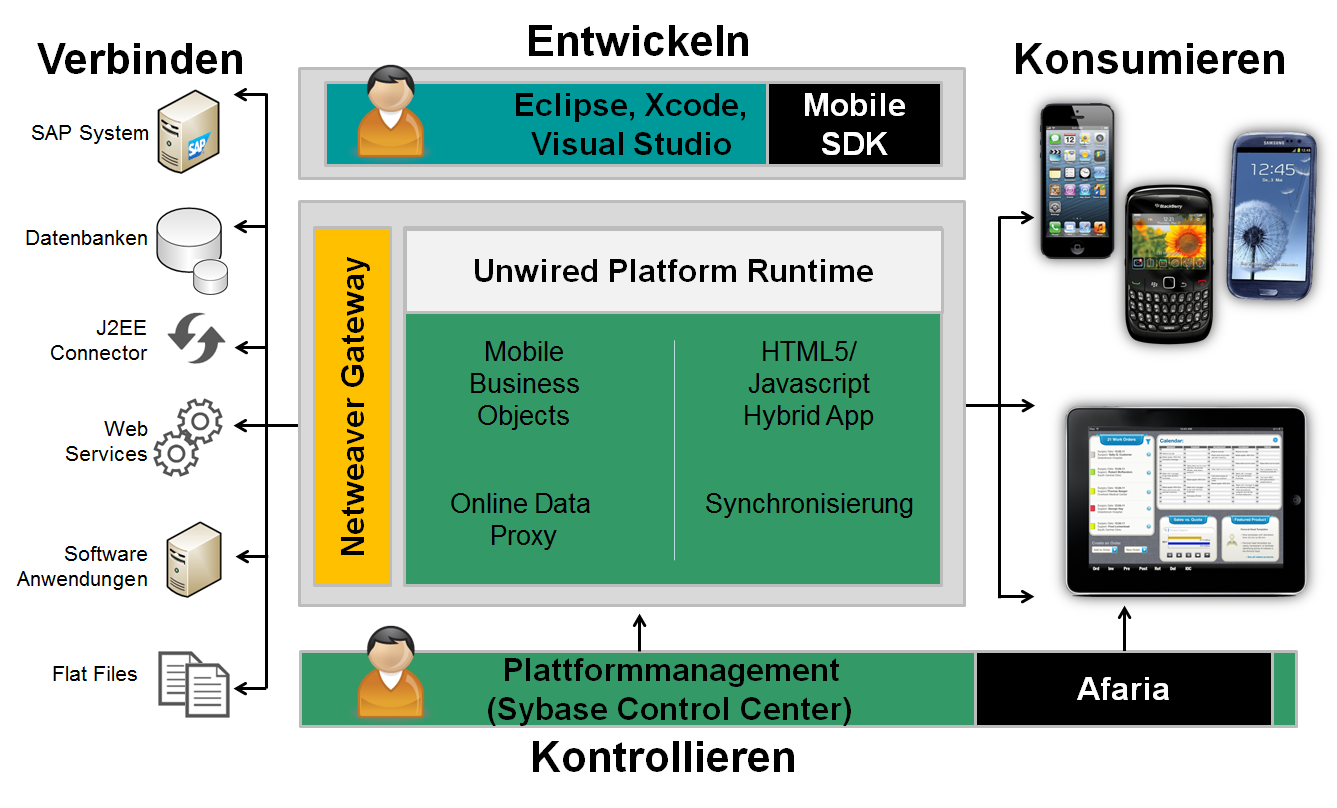
\includegraphics[width=0.9\textwidth]{sup}
\end{lstlisting}

Bei längeren Quellcode-Listings empfiehlt es sich jedoch auf eine externe Datei im Ordner Quellcode zu verlinken und diese einzubauen:
\lstinputlisting[language=HTML]{./Quellcode/Beispiel.html}

Statt dem Package lstlisting, welches direkt auf Tex basiert, kann auch das Package minted verwendet werden.
Dieses Package basiert auf python-pygments und unterstützt weit mehr Sprachkonstrukte als lstlisting.
Um das Paket zu verwenden muss es eingebunden werden und zusätzlich python-pygments installiert sein.
(Dies ist mit im Dockerfile vorhanden. Für die anderen Compile-Methoden, wie das native verwenden von Tex Live findet sich hier die Installationsanleitung für das minted Paket: https://ctan.org/pkg/minted?lang=de)

Damit das kompilieren ohne Python trotzdem möglich ist, ist die Funktion standardmäßig ausgebaut. Deshalb muss zusätzlich in der Datei \begin{verbatim}thesis_main.tex \usepackage{minted} \end{verbatim} wieder einkommentiert werden. 

Minted lässt sich dann ganz ähnlich zu lstlisting verwenden:
\begin{lstlisting}
	\begin{minted}{c}
		int main() {
			printf("hello, world");
			return 0;
		}
	\end{minted}
\end{lstlisting}	

Da der Pfad zu den Abbildungen im Hauptdokument definiert wurde, muss hier nur noch der Name des Bildes ohne Dateiendung stehen (sup).

\begin{figure}[H]
\caption{Titel der Abbildung hier}
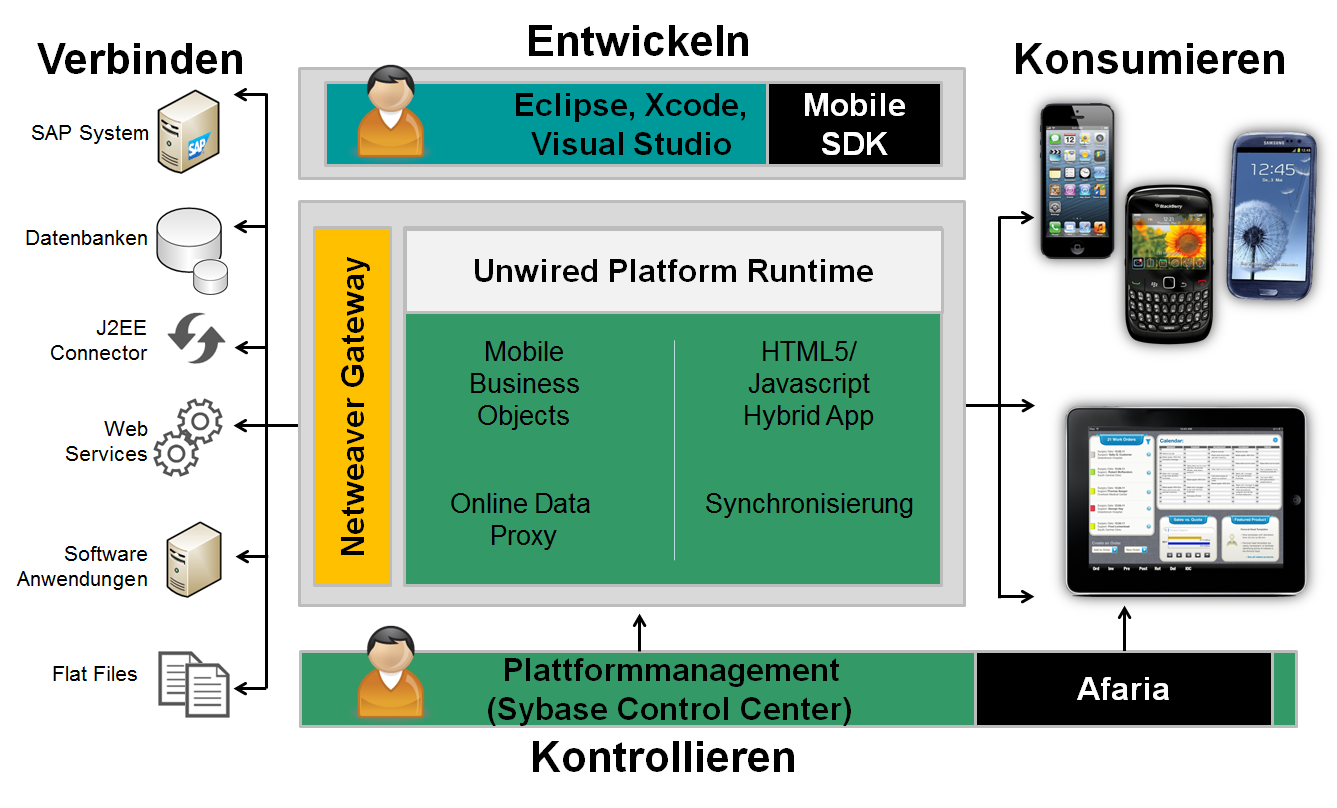
\includegraphics[width=0.9\textwidth]{sup}
\\
Quelle: Eigene Darstellung
\end{figure}

\subsection{Tabellen}
\begin{table}[H]
\caption{Beispieltabelle 1}
\label{tbl:beispieltabelle2}
\begin{tabularx}{\textwidth}[ht]{|l|X|l|}
  \hline
  \textbf{Abkürzung} & \textbf{Beschreibung} & \textbf{Berechnung}\\
  \hline\hline
    MEK & Materialeinzelkosten & \\
  	MGK & Materialgemeinkosten & $+ \uparrow$~*\\
    FEK & Fertigungseinzelkosten & \\
  	FGK & Fertigungsgemeinkosten & $+ \uparrow$~*\\
	SEKF & Sondereinzelkosten der Fertigung & \\
	\hline\hline
	\multicolumn{3}{|l|}{\textbf{= Herstellungskosten}} \\
	\hline\hline
  	VwGK & Verwaltungsgemeinkosten & $+ \uparrow$~*\\
  	VtGK & Vertriebsgemeinkosten & $+ \uparrow$~*\\
  	SEKVt & Sondereinzelkosten des Vertriebes & \\
	\hline\hline
	\multicolumn{3}{|l|}{\textbf{= Selbstkosten}} \\
	\hline\hline
	\multicolumn{3}{|l|}{+ Gewinnaufschlag} \\
	\multicolumn{3}{|l|}{+ Rabatte} \\
	\hline\hline
	\multicolumn{3}{|l|}{\textbf{= Nettoverkaufspreis (NVP)}} \\
	\hline
	\multicolumn{3}{|l|}{+ Umsatzsteuer} \\
	\hline\hline
	\multicolumn{3}{|l|}{\textbf{= Bruttoverkaufspreis (BVP)}} \\
	\hline
\end{tabularx} \\
\cite[Quelle: In Anlehnung an][S. 4]{Beckert.2012}
\end{table}

%\clearpage % hiermit werden alle Bilder Tabellen ausgeworfen

\subsection{Biblatex}
Von den vielen verfügbaren Literatur-Paketen habe ich mich für Biblatex entschieden. Die Anforderungen der FOM sollten hiermit erfüllt sein. Ich habe bisher nur Einträge \enquote{@book} getestet. Wie immer steckt der Teufel hier im Detail und es wird sich später herausstellen, ob Biblatex eine gute Wahl war. Die Anpassungen hierfür liegen unter skripte/modsBiblatex. Ich verwende das Backend Biber, welches bib-Dateien in UTF-8 verarbeiten kann.

In der für den Leitfaden 2018 aktualisierten Version sind außerdem Beispiele für \enquote{online},\footcite[Vgl.][]{website:angular:aboutAngular} also Webseiten, und \enquote{article},\footcite[Vgl.][S. 140]{Decker2009} also wissenschaftliche Artikel, enthalten.

Laut Leitfaden sollen maximal 3 Autoren genannt werden und danach mit
\enquote{et.
al.}
bzw. \enquote{u.a.} ergänzt werden. Damit im Literaturverzeichnis auch nur max.
3 Autoren stehen, muss man beim Füllen der literatur.bib-Datei darauf achten auch nur 3
einzutragen. Weitere Autoren kann man einfach mit \enquote{and others} ergänzen.
Siehe Eintrag für \enquote{Balzert.2008}. Zitiert man dann diese Werk, werden auch in
der Fussnote alle Autoren korrekt genannt wie in dieser
Fußnote\footcite[Vgl.][S.
1]{Balzert.2008} zu sehen ist.\\
Hat man dagegen mehr als 3 Autoren in der bib-Datei hinterlegt, stehen im
Literaturverzeichnis alle drin. In der Fussnote dagegen, steht nur
einer\footcite[Vgl.][S.
1]{Balzert2.2008}, was dem Leitfaden widerspricht.\\
Die Anzahl von 3 wird übrigens über die Option \enquote{maxcitenames=3} des
biblatex-Packages gesetzt. Man muss selbst schauen, dass die Anzahl der Autoren
in den Bib-Dateien mit der Optionseinstellung übereinstimmt.

Diese Fussnote soll zeigen, wie mit einem \enquote{von} vor dem Namen des Autors
umgegangen wird\footcite[Vgl.][S. 1]{Lucke2018}. Man muss für die korrekte
Sortierung eines solchens Namens im Literaturverzeichnis einen \enquote{sortkey}
setzen.

Diese Fussnote soll zeigen, wie mit einer Online-Quelle ohne Jahresangabe
umgegangen wird\footcite[Vgl.][]{Belastingdienst}.

Diese Fußnote\footcite[Vgl.][S.1]{Beckert.2012} ist nur dazu da zu zeigen, wie mit mehreren Quellen des selben Autors aus dem selben Jahr umgegangen wird, wenn das Stichwort gleich bleibt \footcite[Vgl.][S.2]{Beckert.2012.1} oder sich ändert\footcite[Vgl.][S.3]{Beckert.2012.2}. Laut Leitfaden sollte bei gleichem Autor, Jahr und Stichwort ein Buchstabe an die Jahreszahl gehangen werden. Zum Beispiel 2012a. 

\subsection{Abkürzungen}
Abkürzungen werden mithilfe des Pakets Acronym eingebunden. Alle Abkürzungen sollten in der Datei acronyms.tex mithilfe des \begin{verbatim}
	\acro
\end{verbatim} Befehls festgelegt werden. Im Text werden diese dann mit \begin{verbatim}
	\ac{Abkürzung}
\end{verbatim} benutzt. Bei der ersten Verwendung einer Abkürzung wird der Begriff in beiden Formen dargestellt. So wie hier: \ac{WYSIWYG}. Nur wenn eine Abkürzung tatsächlich verwendet wird erscheint sie auch im Abkürzungsverzeichnis.

Sollte es im Abkürzungsverzeichnis zu Anzeigefehlern kommen kann dies daher rühren, dass eine Abkürzung verwendet wird, die länger ist als \ac{WYSIWYG}. In diesem Fall müsst ihr in der Datei acronyms.tex den Parameter [WYSIWYG] durch eure längere Abkürzung ersetzen.

\subsection{Listen und Aufzählungen}
\subsubsection{Listen}
\begin{itemize}
\item ein wichtiger Punkt
\item noch ein wichtiger Punkt
\item und so weiter
\end{itemize}
\subsubsection{Aufzählungen}
\begin{enumerate}
\item Reihenfolge ist hier wichtig
\item Dieser Punkt kommt nach dem ersten
\item Da sollte jetzt eine 3 vorne stehen
\end{enumerate}

\paragraph{Tiefste Ebene 1}
Dies ist die tiefste Gliederungsebene. Sollten doch mehr Ebenen benötigt werden, muss eine andere Dokumentenklasse verwendet werden.

\paragraph{Tiefste Ebene 2}
Der zweite Punkt in dieser Ebene ist zur Erinnerung daran, dass es nie nie niemals nur einen Unterpunkt geben darf.

\subsection{Skript zum Kompilieren}
Latex will ja bekanntlich in einer bestimmten Reihenfolge aufgerufen werden:
\begin{lstlisting}
lualatex thesis_main.tex
biber thesis_main
lualatex thesis_main.tex
lualatex thesis_main.tex
thesis_main.pdf
\end{lstlisting}

Dies ist der Inhalt der Batchdatei \enquote{compile.bat}.

\subsection{PlantUML}

\begin{lstlisting}
\begin{plantuml}
@startuml
Class01 <|-- Class02
Class03 *-- Class04
Class05 o-- Class06
Class07 .. Class08
Class09 -- Class10
@enduml
\end{plantuml}
\end{lstlisting}
